\chapter{検出器 (MAIKo TPC)}
%\section{MAIKo TPC}
\section{MAIKo TPC とは}
Time Projection Chamber (TPC) は荷電粒子の飛跡を検出するために広く用いられている検出器である。
我々は不安定核実験のためにMAIKo TPC を開発した。
図\ref{fig::MAIKo_view}にMAIKo TPC の概観図を示す。
荷電粒子がMAIKo TPC のガス中を通過するときに電子を発生させる。
この電子をドリフト電場により読み出し面にドリフトさせることで飛跡を検出する。
読み出しパッドである$\mu$-PICは図\ref{fig::mupic}のようにanode strip とcathode strip が垂直に配置されている。
anode strip、cathode stripともに400~$\mu$m 間隔で256~chに分割されており、
合計512~chで信号を読み出している。
\begin{figure}
  \centering
  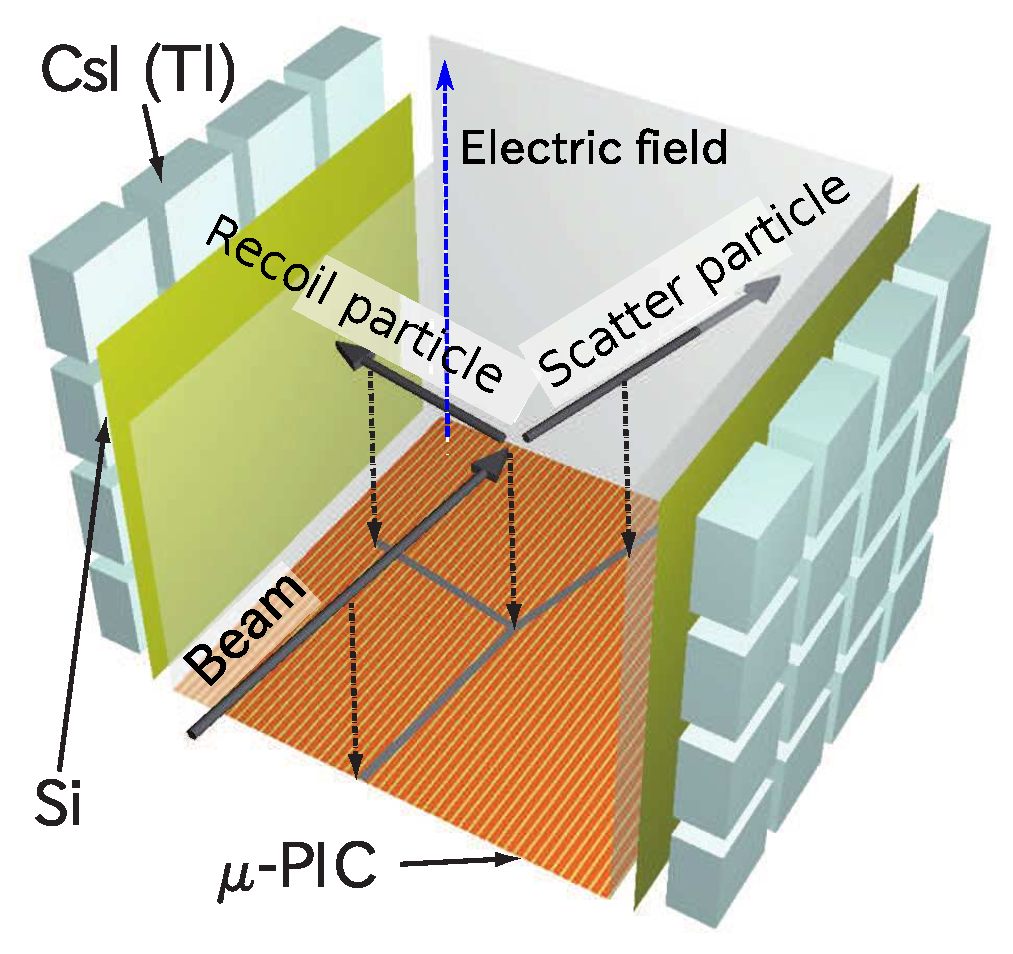
\includegraphics[clip, width=0.7\columnwidth]{eps/at_fig2.eps}
  \caption[MAIKo TPC の概観図。]{MAIKo TPC の概観図。
    図では荷電粒子が入射し、検出器中の粒子と散乱した事象を表している。
  }
  \label{fig::MAIKo_view}
  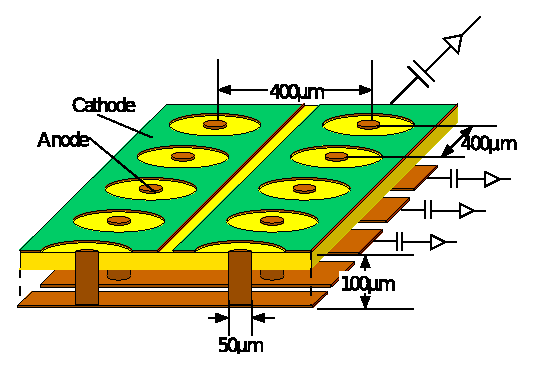
\includegraphics[clip, width=0.7\columnwidth]{eps/upic_struc.eps}
  \caption[$\mu$-PICの概観図。]{$\mu$-PICの概観図。
    図中の横方向にanode strip、奥行き方向にcathode strip が配置されている。
  }
  \label{fig::mupic}
\end{figure}
図\ref{fig::MAIKo_view}中でanode strip は$z$軸、cathode strip は$x$軸と平行である。
ドリフト電場により移動してきた電子をanode strip、cathode strip により読み出し、
それぞれ$x$軸、$z$軸座標を検出することができる。
また、anode strip、cathode strip で検出される信号の時間分布により$y$軸座標を決定することができる。
MAIKo TPC からは図\ref{fig::track_demo}のようにanode strip に垂直な面 ($z-y$平面) に射影された飛跡と
cathode strip に垂直な面 ($z-y$平面) に射影された飛跡の2つの画像が出力される。
anode strip とcathode strip はそれぞれ256~chで構成され、
読み出される信号波高の時間変化は100~MHzで1,024~samples測定される。
そのため、出力される画像の解像度は$256\times1,014$~pixels となる。

\section{検出ガスの決定}
標的には炭素の含まれる炭化水素を用いる。
この実験では低エネルギーの荷電粒子の飛跡を検出するため、
飛跡が比較的長くなるエネルギーロスが小さいガスが適する。
そこで、質量数が最も小さいメタン ($\rm{CH}_{4}$) を用いた。
また、ガスの圧力によって飛跡の長さが変化する。
そこで、$\alpha$粒子の検出効率がよくなるガス圧を求めた。

ガス圧はシミュレーションによって決定した。
${}^{12}\rm{C}$と中性子との散乱をKondoらの実験で求められた
微分断面積の角度分布を用いて再現し、
散乱後に${}^{12}\rm{C}$が$Ex = 7.65\rm{MeV}$に励起し、
${}^{12}\rm{C}\rightarrow{}^{8}\rm{Be}+{}^{4}\rm{He}\rightarrow{}^{4}\rm{He}\times 3$
と崩壊する過程を考えた。
この時、$\alpha$粒子が持つエネルギーの分布は図\ref{fig::alphaenergydist}のようになる。
このような粒子に対して
\begin{enumerate}
\item
  MAIKoの有感領域内 ($102.4\rm{mm}\times 102.4\rm{mm}\times 140\rm{mm}$) で停止する
\item
  飛跡の長さが$20\rm{mm}$以上である
\end{enumerate}
という条件の時に検出可能とすると、検出効率の圧力依存は図\ref{fig::alphaefficiency}のようになる。
図\ref{fig::alphaefficiency}より、$75\rm{hPa}$付近が最も検出効率が高いことが分かる。
そこで、$50\rm{hPa}$、$100\rm{hPa}$の3通りでのオペレートを決定した。

\subsection{ドリフトスピード}
TPCの特性上、ドリフト電場方向のアクセプタンスは電子のドリフトspeedに依存する。
ドリフトケージの大きさ ($140\rm{mm}$) を可能な限り使用するためには、
MAIKo TPC の時間アクセプタンス ($10.24\rm{\mu s}$) で$140\rm{mm}$となるようなドリフトスピード
($140\rm{mm}/10.24\rm{\mu s} \sim 0.0135\rm{mm/ns}$) に調整する必要がある。

\subsection{拡散効果}

\subsection{ガスの種類及び圧力の決定}

\section{MAIKo TPC のオペレート}
\subsection{HV系}
\subsection{ガス系}
\subsection{回路系}
\subsection{電子のドリフト速度}
\subsection{電子の増幅率}

%ドリフト速度の決定方法は30 degree 方向に$\alpha$線源から$\alpha$を出して、
%その飛跡がデータ上でどう見えるかで決定する。
%ドリフト速度の時間依存性も見た。

%\section{中性子カウンター (液体シンチレータ)}
%\subsection{キャリブレーション}
%\subsection{波形弁別}
%\subsection{検出効率}
%
%\section{中性子カウンター (金属箔)}
%
